The application of a stimulus to the nervous system leads to changes determined by
two main properties:
\begin{itemize}
    \item \textbf{Excitability:} the capability of a nerve cell to react to an
    incoming impulse.
    \item \textbf{Plasticity:} certain permanent functional transformations arise in
    particular systems of neurons as a result of appropriate stimuli or their
    combination.
\end{itemize}
The communication between neurons occurs through action potentials, as shown in the
following picture.
\begin{figure}[H]
    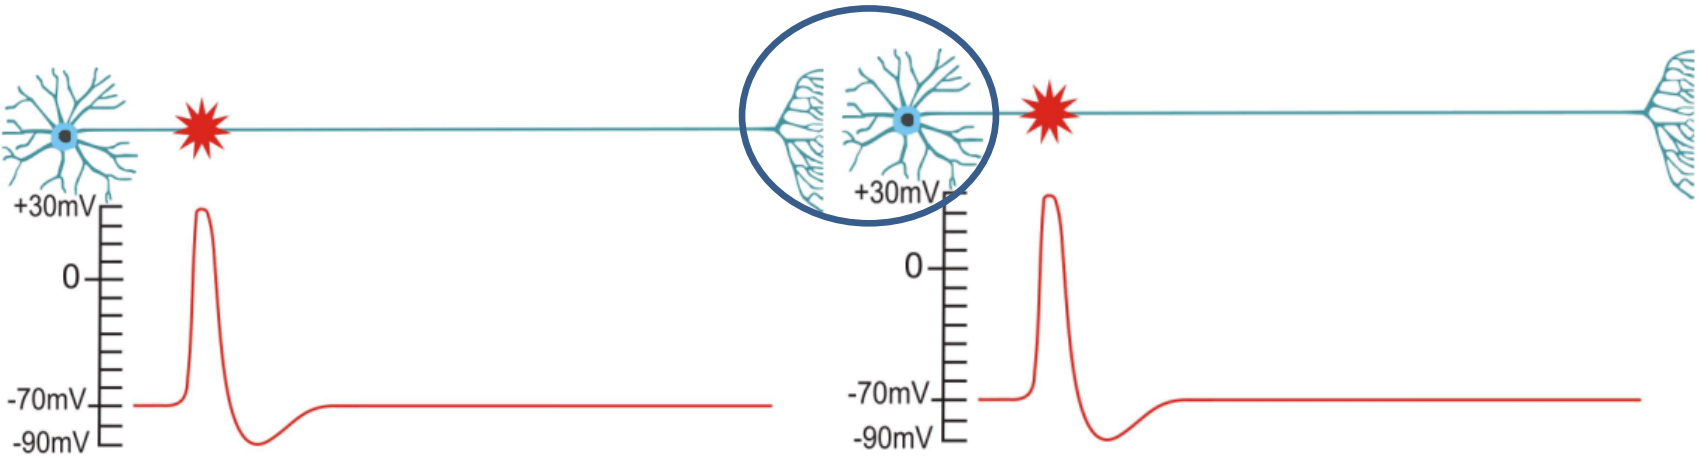
\includegraphics[scale=0.35]{1_1}
    \centering
\end{figure}
Measuring, analyzing, and processing brain signals is done for several reasons, but
the three main ones are listed below:
\begin{itemize}
    \item \textbf{Learn} more about the brain functioning.
    \item \textbf{Mimic} the brain functions in an artificial way - i.e. neuromorphic
    engineering.
    \item \textbf{Employ} brain signals for control and communication, as in the
    case of prosthetics.
\end{itemize}
The nerual code can either be read or written by exploiting several distinct
techniques exhibiting different levels of:
\begin{align*}
    \begin{matrix}
        \textbf{Invasiveness} && \textbf{Risk} &&
        \textbf{Spatial resolution} && \textbf{Temporal resolution}
    \end{matrix}
\end{align*}
The technology nowadays allows fair degrees of spatial and temporal resolution, with
the main reading techniques being fMRI, PET, optical imaging, EEG, ECoG, MEA,
single neuron, and others. Notice that also the number of reading sites is constantly increasing, due to the
exploitation of multiple electrode devices.
\begin{figure}[H]
    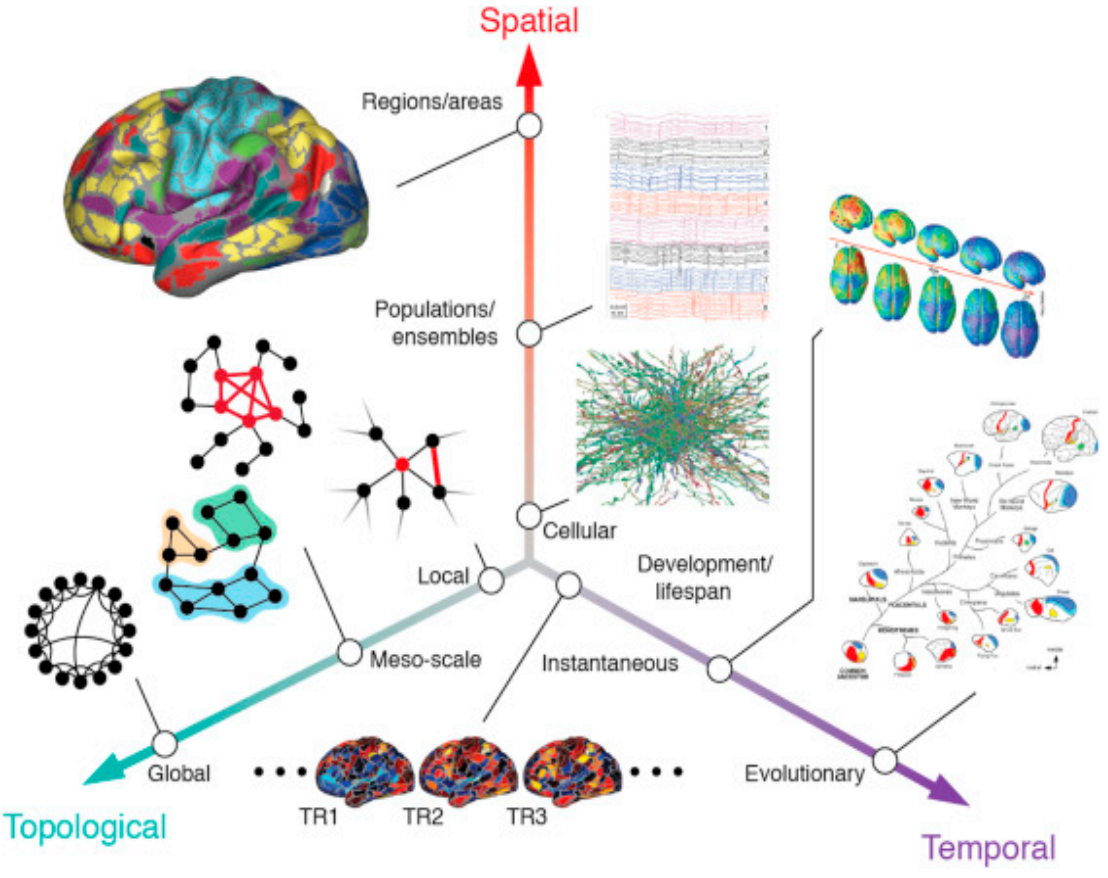
\includegraphics[scale=0.375]{1_2}
    \centering
\end{figure}
The multi-scale brain model presented above aims at showing the different levels at
which the brain activity can be investigated, in terms of spatial, temporal,
and topological scales.
Let's stress once more that the brain can be studied at different level of complexity,
which are somehow related to the risk due to the techniques involved to do so.
\begin{figure}[H]
    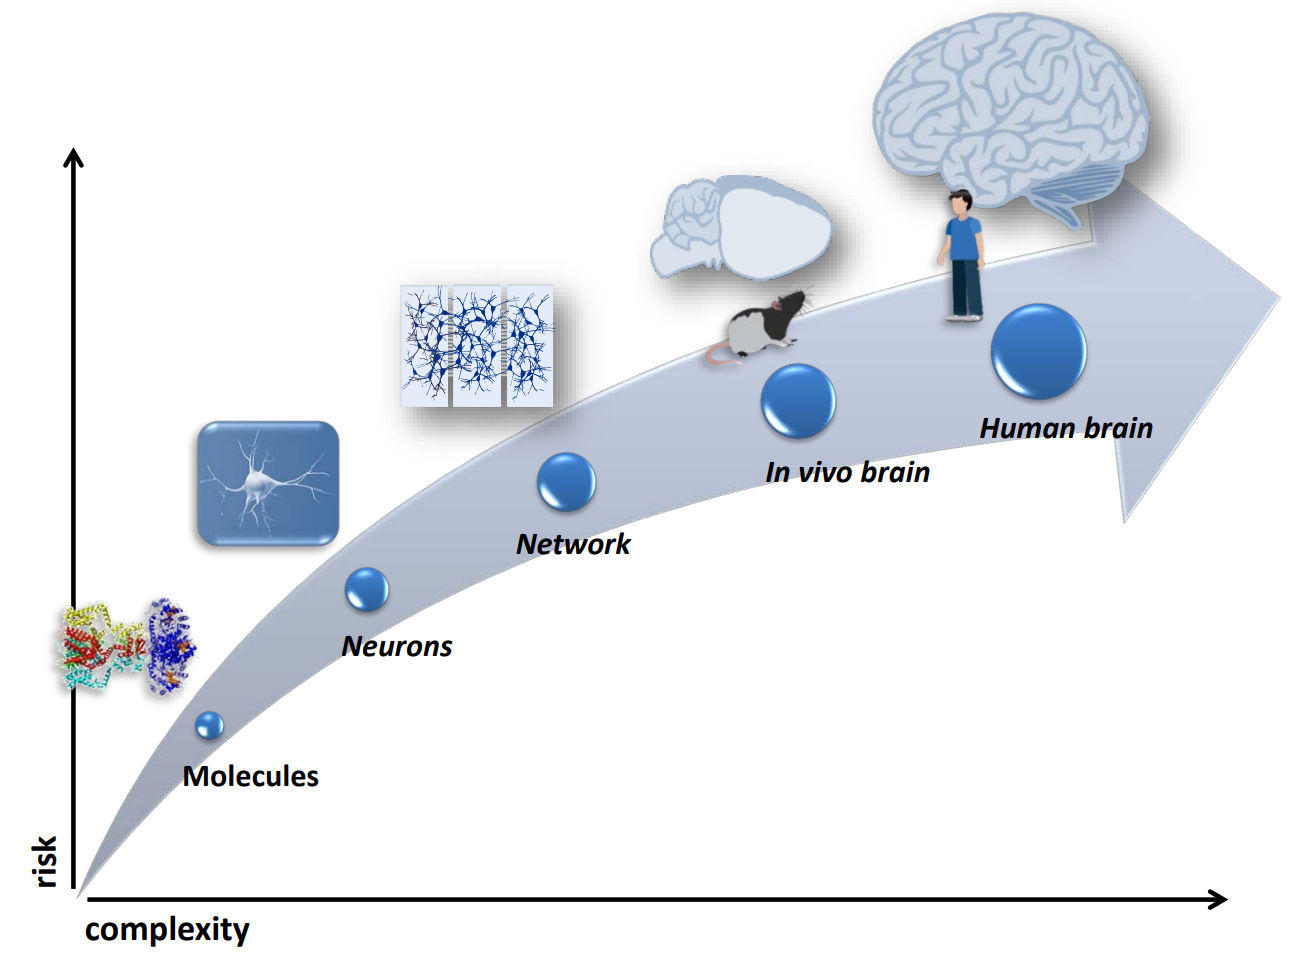
\includegraphics[scale=0.35]{1_3}
    \centering
\end{figure}
Notice that in general the functional unit of the brain is not a single neuron.\\
Two main classes of techniques exist: the \textit{in vitro} and \textit{in vivo} ones. Generally, the
second family is more complex to employ, as it requires not to damage the brain of
the experiment subject. One of the principal technologies to study \textit{in vitro} networks
is MEAs (Micro Electrode Arrays), which are able to detect the activity
of the network at several recording sites and for extended time periods. An issue
related to MEAs is the difficulty often encountered in analysing the recorded data
and interpretating the results in a meaningful way.\\
In general, by recording neural signals at high frequencies and close to few
neurons a signal made of spikes, indicating the firing of a neuron, can be obtained,
while by recording at higher distances the local field potetial (LFP) is instead
obtained, consisting in the low frequency component and accounting for several
neurons as a sort of superposition of their effects.\\
It is common to find in vitro neural networks since they are extensively employed in
research due to their fair level of organization and to the capability to easily
record their activity with arrays of electrodes. Nonetheless, some issues related to
\textit{in vitro} networks are the fact that they have no fidelity w.r.t. \textit{in vivo} neurons,
starting from the fact that they generally arranged in 2D layers, instead of
more complex three-dimensional networks.
\begin{figure}[H]
    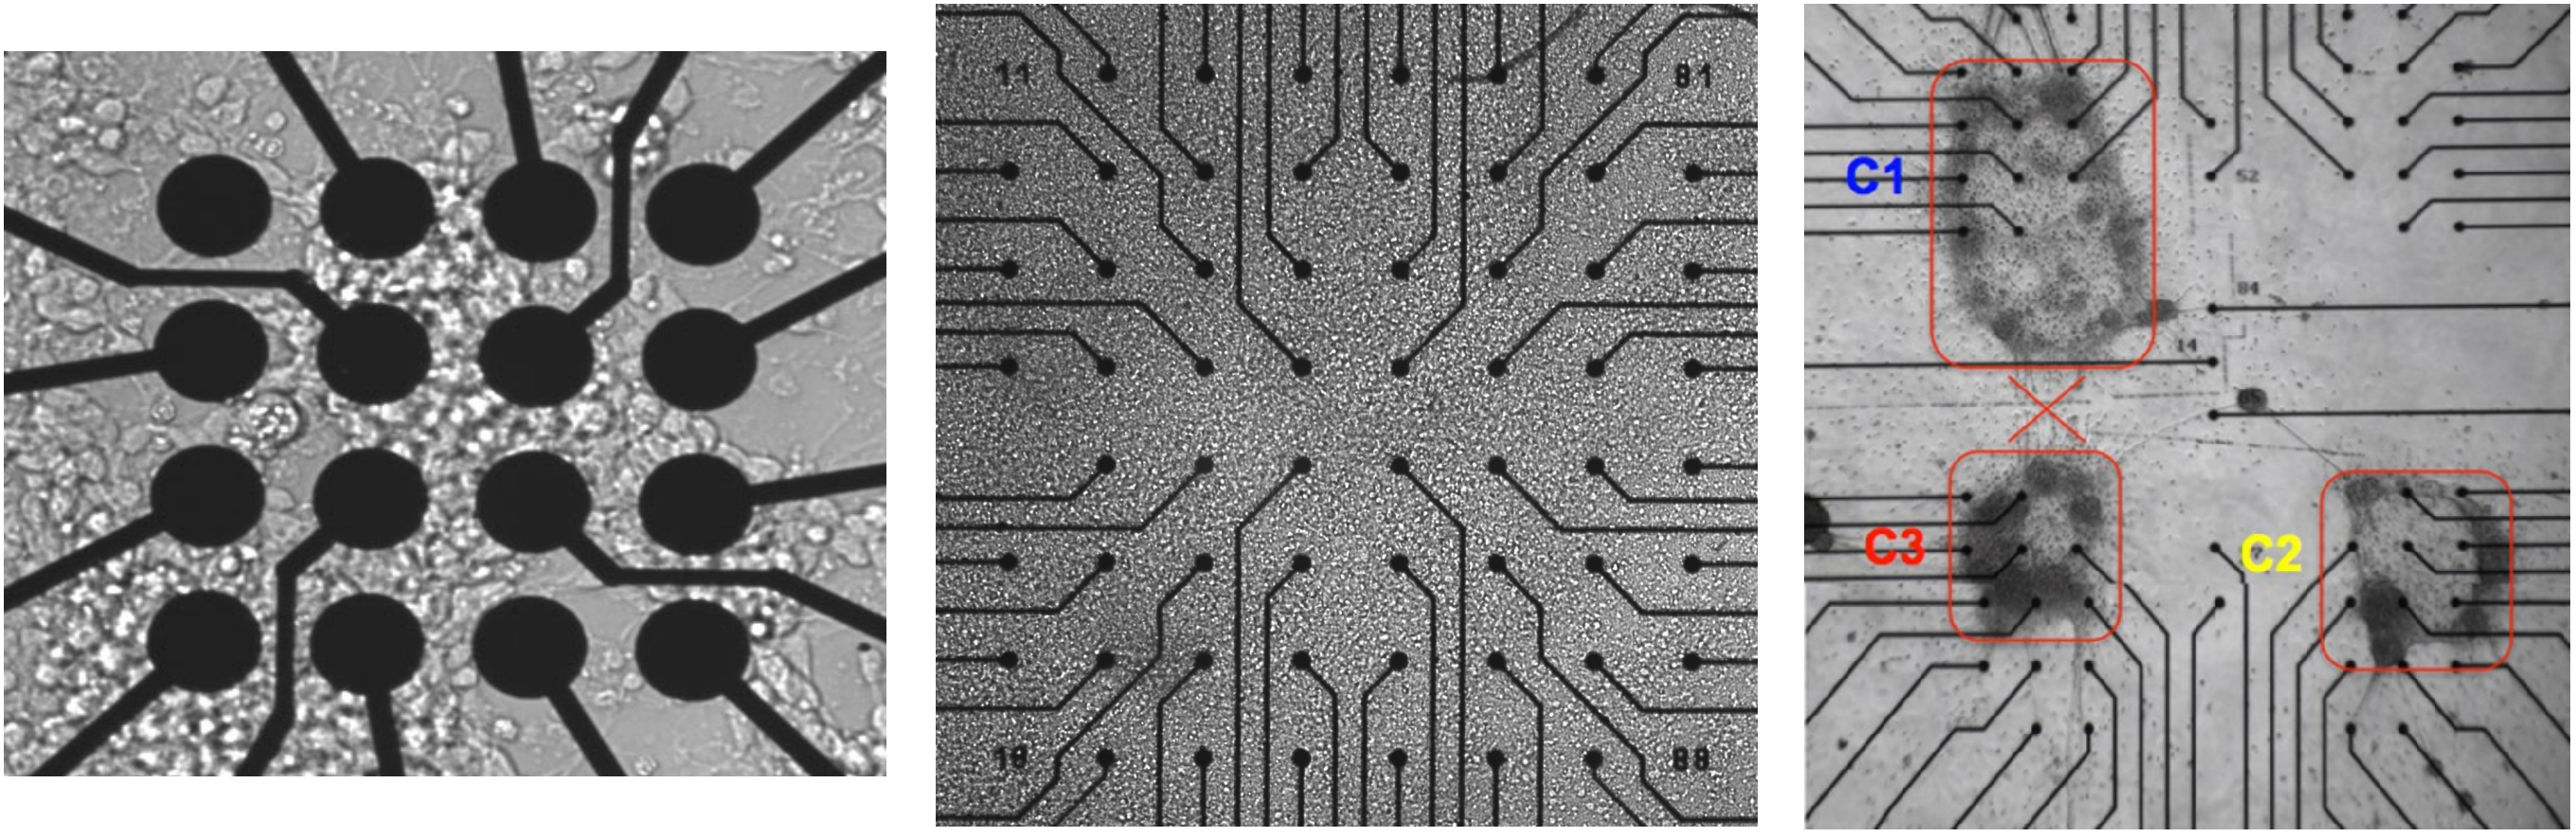
\includegraphics[scale=0.275]{1_4}
    \centering
\end{figure}
Another crucial concept is the one of brain modularity, as a matter of fact the brain
is redundant and intrinsically modular, due to the fact that it is composed of
local networks that are embedded into networks of networks.\\
Other wideley spread techniques are in vitro brain slices and \textit{in vivo} surgical
procedure. In both cases data are collected from biological tissue by means of
MEAs or similar technologies.\\
The analysis of neural signals is usually performed on spike trains, which are
derived by filtering the raw signal recorded from electrodes and by detecting the
spikes present in it. Notice that the crucial point is not the magnitude of a
certain spike, rather its position on the time axis, indicating when it was fired.
\begin{figure}[H]
    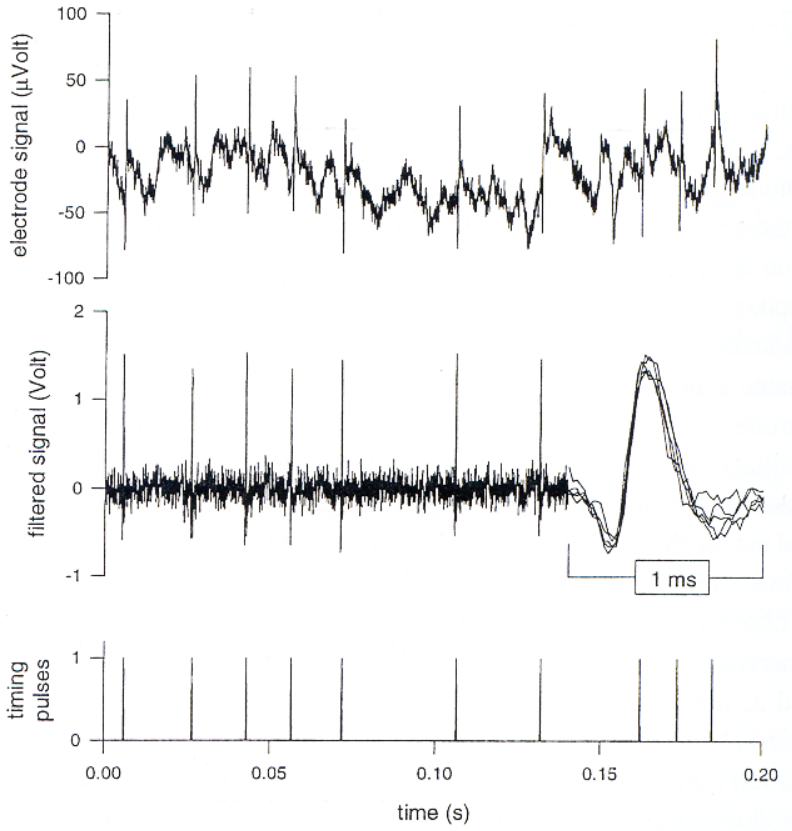
\includegraphics[scale=0.5]{1_5}
    \centering
\end{figure}
It is important to point out that the shape of a spike is highly influenced by the
position of the measuring electrode w.r.t. the neuron that emitted it, enabling
the researchers to recognize all the spikes emitted by the same source - i.e. a
particular neuron - and this is called spike sorting.\\
The main areas of research in this subject are reported in the following list:
\begin{itemize}
    \item Identification and classification of spike events (spike detection and
    spike sorting).
    \item Techniques for measuring the association between neural spike trains.
    \item Quantification of the neural response to a stimulus.
\end{itemize}
Finally, let's highlight that the high number of electrodes employed in today's
research implies a number of new challenges concerning data aquisition, storage,
and analysis.